\chapter{ModLab Modules}
This chapter is \textbf{Work in Progress} and thus subject to change at any time!

Here I wanna give you a brief overview over the modules (no particular order). Each one will be discussed in more detail, so no worries. 

I will also mark everything that is currently just a concept or idea with a (c) behind its name. 

\begin{itemize}
	\item Bus Adapter
	\begin{itemize}
		\item 1:1 Extension of the backplane bus with connector at the front
		\item Termination resistors for differential pairs
		\item LED indicators for supply voltages
	\end{itemize}
%-------------------------
	\item Host-Bus-Controller / HBC
	\begin{itemize}
		\item Brain of the ModLab
		\item Master for all backplane interfaces
		\item 5'' TFT LCD with touch
		\item ESP32 Co-Processor
		\item SD card slot for logging and more
		\item USB interface
	\end{itemize}
%-------------------------
	\item Symmetric Linear Power Supply
	\begin{itemize}
		\item Symmetric regulated Voltage
		\item Both CC and CV modes
		\item Controlled via PWM
	\end{itemize}
%-------------------------
	\item Symmetric Switching Mode Power Supply (c)
	\begin{itemize}
		\item Single regilated Voltage
		\item Both CC and CV modes
		\item Controlled via PWM
	\end{itemize}
%-------------------------
%	\item Linear Power Supply (c)
%\begin{itemize}
%	\item Stromversorgung mit größerer Leistung
%	\item Spannungs- und Stromgeregelt
%	\item Co-Prozessor übernimmt Regelung
%\end{itemize}
%-------------------------
	\item Switching Mode Power Supply
	\begin{itemize}
		\item High-current power supply
		\item Both CC and CV modes
		\item Controlled via PWM
	\end{itemize}
%-------------------------
	\item Waveform Generator Analog (c)
	%\begin{itemize}
	%	\item MAX038 als Generatorbaustein
	%	\item Sinus, Rechteck und Dreieck
	%	\item Ansteuerung eventuell über Co-Prozessor
	%\end{itemize}
%-------------------------
	\item Waveform Generator DDS
	\begin{itemize}
		\item AD9833 Waveform Generator
		\item 0.1Hz to 12.5MHz
		\item Sine wave, triangle and square wave
		\item VCA and Output Driver
	\end{itemize}
%-------------------------
	\item Logic Probe Tester (c)
	%\begin{itemize}
	%	\item Kann Pegel registrieren und gibt Pegelhöhe an
	%	\item Kann Low-Power Rechteck generieren um Signalbahnen zu verfolgen
	%	\item Test-Probes mit Pogo-Pins
	%	\item Tastköpfe aus 3D-Drucker
	%\end{itemize}
%-------------------------
	\item Diode Tester
	\begin{itemize}
		\item 4 different constant current sources
		\item capable of creativ characteristic curves
		\item Co-Prozessor übernimmt Regelung
	\end{itemize}
%-------------------------
	\item Electronic Load
	\begin{itemize}
		\item Resistive Load for up to 15A
		\item Two Channels
		\item Load Limiter with thermocouple on Heatsink
	\end{itemize}
%-------------------------
	\item Speaker Module (c)
	%\begin{itemize}
	%	\item Signaltöne für verschiedene Angelegenheiten
	%	\item Hochgefahren, Störung, Durchgang etc...
	%	\item zwei Lautsprecher, einer für Melodie, einer für Signal
	%\end{itemize}
%-------------------------
	\item Oscilloscope
	%\begin{itemize}
	%	\item China Einkanal-Oszi auf Eurokarte portiert
	%	\item Für schnelle Tests von langsamen Signalen
	%\end{itemize}
%-------------------------
\end{itemize}

%------------------------------------------------------------------------------------------------------------------------

\section{Bus Adapter}
The Bus Adapter is one of the first modules. It's main function is to terminate the differential bus lanes. For this reason the Bus Adapter is made twice to terminate each end of the backplane. 

Also it serves as an extension to the backplane, since each module has a connector on its front panel serving as a 1:1 connection to the backplane. This way the slot doesn't get wasted for nearly no function.

In addition to that, each supply voltage has a dedicated LED to show if the voltage is available or if a fuse has blown. 

And that is all there is to it. 

%------------------------------------------------------------------------------------------------------------------------

\section{Host Bus Controller}
The Host Bus Controller (HBC) is the heart of the ModLab. It acts as master for the backplane busses as well as user interface. Since it is quite a busy module, I'll try my best to explain each function seperately

\begin{figure}[H]
	\centering
		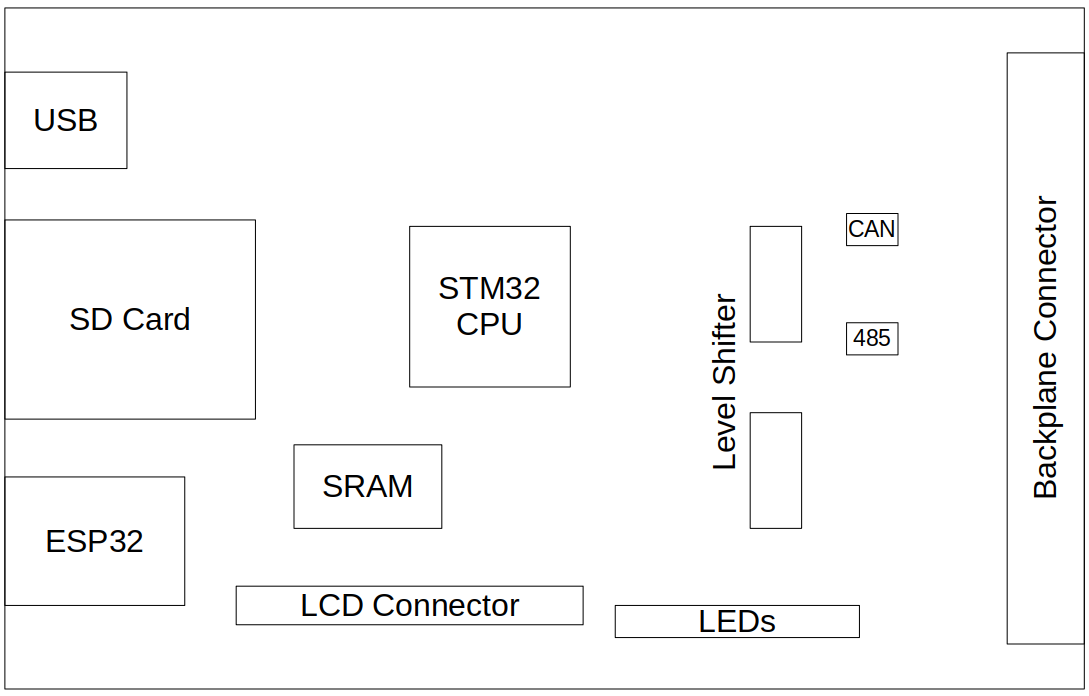
\includegraphics[width=\textwidth]{pictures/overview_cpu.png}
	\caption{PCB Overview HBC}
	\label{img:HBC}
\end{figure}

\subsection{CPU}

The core of the HBC is the STM32F767 microcontroller. It controls everything in the entire system and provides the user interfaces. 

With 2MB of Flash and 512kB RAM it has more than plenty of storage both for the program code as well as process data and variables. Also at 216MHz max clock rate it is really fast and can process everything in a timely manner. At least that was the thought behind choosing this chip. 

\subsection{Additional Hardware}

Also it has a lot of interfaces which are used on the PCB. Additionally to the interfaces mentioned in chapter 5.4, internally the module has two SPI busses, one for the touch controller and one for the ESP32 coprocessor. A USB interface for debugging and monitoring is inlcuded as well. 

For logging and config storage I included an SD card slot. 

The FSMC (Flexible SRAM Memory Controller) interface of the microcontroller is connected to an external 512k x 16 SRAM chip. I thought about including an external flash memory for application software, but decided against it, since the internal flash seemed more than enough. The external SRAM might come in handy tho if I decide to build modules like logic analyzers which have a ton of data coming in at once. 

The ESP32 module will provide a webinterface for monitoring and diagnosis, but not for controlling the system. This decision was made from a security stand point. 

For Interfacing with the whole system, a 5" Nextion TFT LCD is connected via UART. 

How the protocols on the interfaces will look like, will be discussed in another chapter. 

%------------------------------------------------------------------------------------------------------------------------

\section{Diode Tester}
The Diode Tester is actually quite simple in design. It consists of 4 constant current sources which are tuned to about 2.2mA, 5mA, 10mA and 20mA respectively. Due to this I can enable up to 16 different currents through the Device Under Test (DUT) and even make a crude characteristic curve out of it. 
Following is a simplified schematic of the current sources.

\begin{figure}[H]
	\centering
		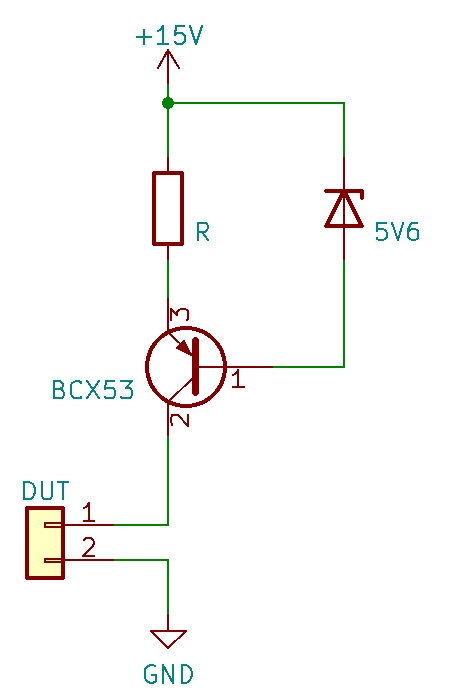
\includegraphics[width=5cm]{pictures/cc_source.png}
	\caption{Current Source Schematic}
	\label{img:CC_Diode}
\end{figure}

The current is configured via the resistor according to Kirchhoff's loop rule. $U_{be}$ of the transistor is typically 0.7V, which means the voltage across the resistor is fixed at $5.6V - 0.7V = 4.9V$. With the values of 2.2k, 1k, 499 and two 499 in parallel respectively, the following currents are available:

\begin{align*}
	\frac{4.9V}{2.2 k\Omega} & = 2.22 mA\\
	\frac{4.9V}{1 k\Omega}  & = 4.9  mA\\
	\frac{4.9V}{499 \Omega} & = 9.81 mA\\
	\frac{4.9V}{249.5 \Omega} & = 19.63 mA\\
\end{align*}

In V1 I tried to enable the sources via a P-channel MOSFET, which for some strange reason didn't work. So I decided for V2 to use small reed relais I had in storage. 

\vspace{1cm}

The module also has an STM32F103 controller on board which is connected to the backplane via CAN and I2C. I did both since I hadn't yet decided which interface I am going to use for the module. 

\subsection{Parameters}
\begin{table}[H]
    \centering
    \begin{tabular}{|c|c|l|}
        \hline
        \textbf{No.}   &   \textbf{Size} & \multicolumn{1}{|c|}{\textbf{Description}}\\ \hline \hline
        10h   &  2 Byte & DUT Voltage at 2 mA \\ \hline
		11h   &  2 Byte & DUT Voltage at 5 mA \\ \hline
		12h   &  2 Byte & DUT Voltage at 7 mA \\ \hline
		13h   &  2 Byte & DUT Voltage at 10 mA \\ \hline
		14h   &  2 Byte & DUT Voltage at 12 mA \\ \hline
		15h   &  2 Byte & DUT Voltage at 15 mA \\ \hline
		16h   &  2 Byte & DUT Voltage at 17 mA \\ \hline
		17h   &  2 Byte & DUT Voltage at 20 mA \\ \hline
		18h   &  2 Byte & DUT Voltage at 22 mA \\ \hline
		19h   &  2 Byte & DUT Voltage at 25 mA \\ \hline
		1Ah   &  2 Byte & DUT Voltage at 27 mA \\ \hline
		1Bh   &  2 Byte & DUT Voltage at 30 mA \\ \hline
		1Ch   &  2 Byte & DUT Voltage at 32 mA \\ \hline
		1Dh   &  2 Byte & DUT Voltage at 35 mA \\ \hline
		1Eh   &  2 Byte & DUT Voltage at 37 mA \\ \hline
		20h   &  1 Byte & Starting Current	\\ \hline
		21h   &  1 Byte & Ending Current \\ \hline
    \end{tabular}
	\caption{Diode Tester Parameter List}
\label{tab:Par-Diode}
\end{table}
\subsection{Operation Modes}
Start Measurement with ``Enable Output'' Command.

\begin{table}[H]
    \centering
    \begin{tabular}{|c|c|l|}
        \hline
        \textbf{Mode}   &  \multicolumn{1}{|c|}{\textbf{Description}}\\ \hline \hline
        0   &  \makecell[l]{Single Value Measurement \\ Starting Current only}\\ \hline
		1   &  \makecell[l]{Coarse Characteristic Curve \\ Starting Current to Ending Current \\ Only Hardware Sources enabled}\\ \hline
		2   &  \makecell[l]{Medium Characteristic Curve \\ Starting Current to Ending Current \\ Every other possible current}\\ \hline
		3   &  \makecell[l]{Fine Characteristic Curve \\ Starting Current to Ending Current \\ Every possible current}\\ \hline
    \end{tabular}
	\caption{Diode Tester Parameter List}
\label{tab:Modes-Diode}
\end{table}
\subsection{Channels/Outputs}
Enabled Channels:
\begin{itemize}
	\item ADC0
\end{itemize}
\section{Waveform Generator DDS}
For most of the design I have to thank ``Daumemo'' from \textcolor{blue}{\href{https://daumemo.com}{daumemo.com}}. I wanted to use the AD9833 waveform generator IC and his guide helped me design the circuit around it. 

The board mainly consists of the STM32F103 controller, the AD9833 signal generator, a VCA (voltage controlled amplifier) and an output amplifier. Gain and Offset are controlled via PWM, the Interface to the AD9833 is SPI. 

The Signal Generator is capable of generating Sine, Triangle and Square waves from 1Hz up to 12.5MHz with a 1Hz resolution. 

\subsection{Parameters}
\begin{table}[H]
    \centering
    \begin{tabular}{|c|c|l|}
        \hline
        \textbf{No.}   &   \textbf{Size} & \multicolumn{1}{|c|}{\textbf{Description}}\\ \hline \hline
        10h   &  4 Byte &  Set Frequency [1Hz]\\ \hline
		20h   &  2 Byte &  Set Vout Peak-Peak [0.1V]\\ \hline
		30h	  &  2 Byte &  Offset Voltage [0.1V] \\ \hline
    \end{tabular}
	\caption{AD9833 Parameter List}
\label{tab:Par-Waveform9833}
\end{table}
\subsection{Operation Modes}
\begin{table}[H]
    \centering
    \begin{tabular}{|c|c|l|}
        \hline
        \textbf{No.}   & \multicolumn{1}{|c|}{\textbf{Description}}\\ \hline \hline
        0h   &  Square Wave\\ \hline
		1h   &  Sine Wave\\ \hline
		2h	 &  Triangular Wave \\ \hline
    \end{tabular}
	\caption{AD9833 Waveforms List}
\label{tab:mode-Waveform9833}
\subsection{Channels/Outputs}
\section{Symmetric Linear Power Supply (SymPSU)}
The design for the symmetric power supply is derived from the user ``The Big One'' over on \textcolor{blue}{\href{https://hackaday.io/project/4154-bench-power-supply}{Hackaday}}. I adopted it to my STM32 controller and to 3V3 supply voltage. Also I switched the control voltage generation from a dedicated DAC to the PWM-channels of the STM32. I am using the internal ADC on the STM32 as well. 

With these design changes, the SymPSU can provide the following voltages:
\begin{itemize}
	\item Positive voltage
	\begin{itemize}
		\item 0 to 12V @ 0 to 1.2A
	\end{itemize}
	\item Negative voltage
	\begin{itemize}
		\item 0 to -12V @ 0 to 1.2A
	\end{itemize}
\end{itemize}

After tweaking the code, I programmed the following resolutions:

\begin{itemize}
	\item Voltages
	\begin{itemize}
		\item 10 mV / step
	\end{itemize}
	\item Currents
	\begin{itemize}
		\item 0.1 mA / step
	\end{itemize}
\end{itemize}

I am quite happy with these specs, but will likely tweak the design in the future a bit. I still have some issues that are currently fixed in software, rather than in hardware. 

\subsection{Parameters}
\begin{table}[H]
    \centering
    \begin{tabular}{|c|c|l|}
        \hline
        \textbf{No.}   &   \textbf{Size} & \multicolumn{1}{|c|}{\textbf{Description}}\\ \hline \hline
        10h   &  2 Byte &  Set Positive Voltage [mV]\\ \hline
		11h   &  2 Byte &  Set Positive Current [mA]\\ \hline
		12h   &  2 Byte &  Set Negative Voltage [mV]\\ \hline
		13h   &  2 Byte &  Set Negative Current [mA]\\ \hline
		20h   &  2 Byte &  Measured Positive Voltage [mV]\\ \hline
		21h   &  2 Byte &  Measured Positive Current [mA]\\ \hline
		22h   &  2 Byte &  Measured Negative Voltage [mV]\\ \hline
		23h   &  2 Byte &  Measured Negative Current [mA]\\ \hline
    \end{tabular}
	\caption{SymPSU Parameter List}
\label{tab:Par-SymPSU}
\end{table}
\subsection{Operation Modes}
n/a.
\subsection{Channels/Outputs}
Enabled Channels:
\begin{itemize}
	\item ADC0
	\item ADC1
	\item ADC2
	\item ADC3
	\item PWM0
	\item PWM1
	\item PWM2
	\item PWM3
	\item Output Relais
\end{itemize}

\section{Switching Mode Power Supply}
This Power Supply is based on a TL494 PWM Control Circuit. The PWM Controller is getting the reference voltages for Output Voltage and Current from the STM32 via filtered PWM signals. This way a complicated and possibly slow and inaccurate software PID regulator is avoided while the circuit complexity is held at a minimum. A voltage divider is generating the feedback voltage, while a high-current shunt and differential amplifier is generating the feedback voltage for the current. 

The following specs were set for Rev 1. This module will need a redesign in order to fix some mistakes.

\begin{itemize}
	\item Voltage
	\begin{itemize}
		\item 2 .. 22 V Output
		\item 10 mV resolution
	\end{itemize}
	\item Current
	\begin{itemize}
		\item 0 .. 5 A Output
		\item 10 mA resolution
	\end{itemize}
\end{itemize}

\subsection{Parameters}
\begin{table}[H]
    \centering
    \begin{tabular}{|c|c|l|}
        \hline
        \textbf{No.}   &   \textbf{Size} & \multicolumn{1}{|c|}{\textbf{Description}}\\ \hline \hline
        10h   &  2 Byte &  Set Voltage [10mV]\\ \hline
		11h   &  2 Byte &  Set Current [10mA]\\ \hline
		20h   &  2 Byte &  Measured Voltage [10mV]\\ \hline
		21h   &  2 Byte &  Measured Current [10mA]\\ \hline
    \end{tabular}
	\caption{SMPS Parameter List}
\label{tab:Par-SMPS}
\end{table}

\subsection{Operation Modes}
n.a.
\subsection{Channels/Outputs}
Enabled Channels:
\begin{itemize}
	\item ADC0
	\item ADC1
	\item PWM0
	\item PWM1
	\item Output Relais
\end{itemize}